\documentclass[10pt,letterpaper]{article}
\usepackage[utf8x]{inputenc}
\usepackage{amsmath}
\usepackage{amsfonts}
\usepackage{amssymb}
\usepackage{graphicx}
\usepackage{lmodern}
\usepackage[hidelinks]{hyperref}
\usepackage{pgf}
\usepackage{pgfplots}
\usepackage{tabularx}
\pgfplotsset{compat=1.16}
\usepackage[american, nooldvoltagedirection, siunitx, americanvoltages]{circuitikz}
\usetikzlibrary{fit}

\usepackage[
type={CC},
modifier={by-sa},
version={4.0},
]{doclicense}

%\usepackage[left=2cm,right=2cm,top=2cm,bottom=2cm]{geometry}
\author{Scott Howard (KD9PDP)}
\date{}
\title{\footnotetext{\doclicenseThis}QCX Class E Amplifier Design: Practical Equations and Theoretical Derivation}
\begin{document}
\maketitle

\section{Intro}
The QCX is a great amateur radio QRP platform developed by \url{https://qrp-labs.com} with a unique design philosophy. It performs remarkably well ($>80\%$ efficiency and $>\SI{3}{\watt}$ output power) while also not following traditional design rules. Instead, the inventor (Hans Summers, G0UPL) used a trial-and-error approach to make a working amplifier. This document shows how theoretical analysis arrives at the correct (and even slightly more efficient) values right away without trial and error. First, I'll show the conclusions followed by the detailed derivation for those that are interested.

\section{Comparing Original QCX Design to the New Theory}
Nearly all amateur radio QRP Class E amplifiers look like Figure \ref{ClassEnocurrents}. Some square wave signal modulates the gate of a MOSFET. The drain is biased through an inductor $L_1$ and connected to ground through $C_1$. Gate modulation causes voltage modulation at the drain. Filters are used to extract the RF signal you would like to apply to your load resistor $R_L$ (i.e., your antenna).


\begin{figure}
\centering
\begin{circuitikz}
\draw
(0,0) node[nigfetd](fet){}
(fet.D) -- (0,1) to[short,] (1,1) to[short] (3,1) to[L=$L_1$, *-] (3,3)
  node[vcc](VCC){$V_{CC}$};
  \draw (3,1) node[below]{$v_c$};
  \draw (fet.S) -- (0,-1) node[ground]{};
  \draw (fet.G) to[sqV] (fet.G -| -2,-2) -| (-2,-1)
  node[ground]{};
  \draw (1,1) to[C=$C_1$] (1,-1) node[ground]{};
  \draw (3,1) to[short] (4,1)
  to[bandpass, l=Filter, name=filter] (6,1) -- (7,1) to[R=$R_L$, name=RL] (7,-1)
  node[ground](gnd){};
  \node[rectangle, draw, dashed, fit=(RL) (filter) (filterlabel) (RLlabel) (gnd)](box){};
  \node [above] at (box.north) {Typology Specific};
\end{circuitikz}
\caption{Generic Class E Amplifier}
\label{ClassEnocurrents}
\end{figure}

The QCX Class E amplifier uses the filter seen in Figure \ref{ClassEqcx}. The filter was chosen to be a well known filter from the G-QRP club's technical pages, originally designed by Ed Whetherhold (W3NQN). Table \ref{qcxtable} shows the values used for a 7.1 MHz (40 m) QCX transmitter. The ``QCX Start" is the design philosophy in the QCX manual, ``QCX Final" is what was finally realized after experimental optimization, ``NEW Theory" is based on the new theory presented here. In these tables, $\omega$ is the design frequency in radians/sec.

\begin{figure}
\centering
\begin{circuitikz}
  \draw (3,1) node[left]{$v_c$} to[C=$C_f$,o-]
  (5,1) to[L=$L_2$, name=Lf]
  (7,1) to[C=$C_3$]
  (7,-1) node[tlground]{};
  \draw  (7,1) to[L=$L_3$] (9,1) to[C=$C_4$] (9,-1) node[tlground]{};
  \draw (9,1) to [L=$L_4$] (11,1) 
  to[C=$C_5$] (11,-1) node[tlground]{};
  \draw (11,1) -- (12.5,1) to[R=$R_{ant}$] (12.5,-1) node[tlground]{};
  \draw (5,1) to[C=$C_2$] (5,-1) node[tlground]{};
\end{circuitikz}
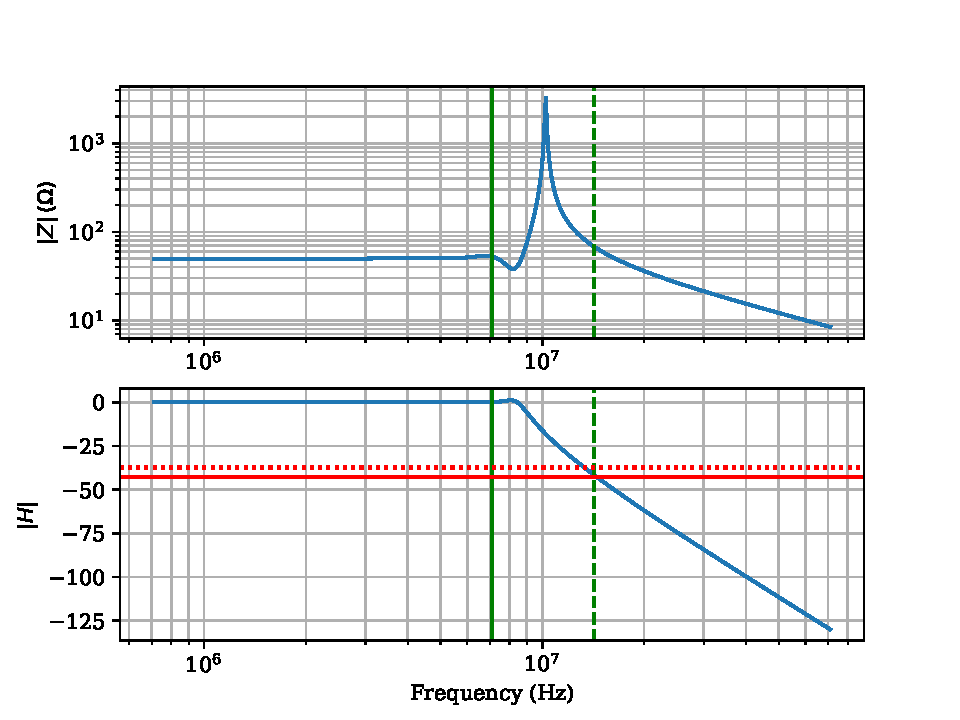
\includegraphics[width=.8\textwidth]{QCXfilt.pdf}
\caption{QCX LPF Class E for 7.1 MHz. It is completely real at $\omega$ (green line) and $2\omega$ (dashed green line).}
\label{ClassEqcx}
\end{figure}



\begin{table}
\centering
%\begin{tabularx}{0.9\textwidth}{cc|ccc}
\begin{tabular}{c|ccc}
& QCX Start & QCX Final & NEW Theory  \\
\hline
\hline 
%Std. & & 10 & $\SI{13}{\micro\henry}$ & 27 dB & 1.5 W & 94\%\\
$\eta$ & 72.2\% & 84.7\% & 87.6\% \\ \hline
$\left\langle P_{out} \right\rangle$ & $\SI{2.3}{\watt}$ & $\SI{3.5}{\watt}$ & $\SI{3.0}{\watt}$ \\ \hline
$L_1 (\SI{}{\micro\henry})$ & 1.12 & 1.00 & 1.12 \\\hline
$C_1 (\SI{}{\pico\farad})$ & 448 & 56 & 112 \\ \hline
$C_f (\SI{}{\nano\farad})$ & 100 & 100 & 100 \\ \hline
$C_2 (\SI{}{\pico\farad})$ & 270 & 270 & 270 \\ \hline
$L_2 (\SI{}{\micro\henry})$ & 1.38 & 1.38 & 1.38 \\ \hline
$C_3 (\SI{}{\pico\farad})$ & 680 & 680 & 680 \\ \hline
$L_3 (\SI{}{\micro\henry})$ & 1.7 & 1.7 & 1.7\\ \hline
$C_4 (\SI{}{\pico\farad})$ & 680 & 680 & 680 \\ \hline
$L_4 (\SI{}{\micro\henry})$ & 1.38 & 1.38 & 1.38 \\ \hline
$C_5 (\SI{}{\pico\farad})$ & 270 & 270 & 270 \\ \hline
\end{tabular}
\caption{ngSpice models results of Class E amplifiers (using 3 parallel BS170 transistors). $f=\SI{7.1}{\mega\hertz}$ $V_{CC}=\SI{12}{\volt}$, $R_{ant}=\SI{50}{\ohm}$. The theoretical starting point according to the QCX manual is ``QCX Start." After the starting point goes through experimental optimization, the ``QCX Final" is the final is what is sold. ``NEW Theory" is based on the derivations in this document. The filters are based on W3NQN's filters from G-QRP}\label{qcxtable}
\end{table}

\section{The New QCX Analytical Design Equations}
QCX Class E amplifier is fundamentally different than pretty much any standard QRP Class E amplifier you'll find. As such, it has different design equations. Table \ref{designcomparetable} compares the design equations for a traditional $R_f$ choke Class E amplifier to the QXC amplifier.


\begin{table}
\centering
%\begin{tabularx}{0.9\textwidth}{cc|ccc}
\begin{tabular}{c|cc}
& Std. Class E Theory & NEW QCX Theory \\
\hline
\hline 
%Std. & & 10 & $\SI{13}{\micro\henry}$ & 27 dB & 1.5 W & 94\%\\
$\left\langle P_{out} \right\rangle \times R_L/V_{CC}^2$ & 0.58 & 1.44 \\ \hline
$L_1 \times \omega/ R_L$ & $\gg 2.84$ & 1.18 \\ \hline
$C_1 \times \omega R_L$ & 0.184 & 0.212 \\ \hline
$C_f \times \omega R_L$ & $Q$ & $ \gg 1$ \\ \hline
\end{tabular}
\caption{Comparison of Design Values. NEW Theory is for a perfect filter. See text for equations for realistic filters.}\label{designcomparetable}
\end{table}

Table \ref{designcomparetable} illustrates the differences between design values. The table assumes an infinitely good filter. More formally, the QCX theoretical design values are based on the impedance of the filter at the second harmonic $Z(2\omega)=\Re\{Z(2\omega\}+i\Im\{Z(2\omega)\}$ and are derived in Section \ref{qcxdesign} and summarized below.


If $Z(2\omega)$ is entirely real (which is the case in the QCX design on \url{https://qrp-labs.com} and $Z(2\omega)=\Re\{Z(2\omega)\}\approx\SI{68}{\ohm}$) and the load resistance is just the antenna $R_L=R_{ant}$:
\begin{align*}
L_1&=\frac{3 \pi R_L Z(2\omega) }{[2R_L+8Z(2\omega)]\omega}
& C_1&=\frac{1}{L_1 (2\omega)^2}\\
C_f &\gg \omega R_L \text{ and } C_f \gg C_1
& \left\langle P_{out} \right\rangle & = \frac{128}{9\pi^2}\frac{V_{CC}^2}{R_L}
\end{align*}

There's actually a different set of design equations for when $C_1 \ll C_f \ll \omega R_{ant}$ that does some cool stuff. The current through the load becomes a cosine (since the load becomes capacitive at $\omega$, and you get increased efficiency $\eta \approx 90\%$ at the cost of lower power ($\approx \SI{1}{W}$ total output on average). It's not derived here, but it's possible to do derive changing some steps later on. It's possibly a much less stable circuit, so I won't spend time on it, but theoretically possible nonetheless.

Finally, the theory presents a completely different strategy for what's required of filters. See Table \ref{filtercomparetable}. It turns out that the filter in Figure \ref{ClassEqcx} is one of the few filter designs that actually meets the requirements! It has an entirely real impedance at $\omega$ and $2\omega$ and presents as a capacitive load for $n\omega$ for $n>2$!

\begin{table}
\centering
%\begin{tabularx}{0.9\textwidth}{cc|ccc}
\begin{tabular}{c|cc}
Impedance & Std. Class E & NEW QCX Theory \\
\hline
\hline 
%Std. & & 10 & $\SI{13}{\micro\henry}$ & 27 dB & 1.5 W & 94\%\\
DC & $\infty$ & $\infty$ \\ \hline
$\omega$ & Complex inductive load & Real load \\
& $R_L+i\omega \Delta L$ & $R_L$\\ \hline
$2\omega$ & $\infty$ & Completely real or $\infty$ \\ \hline
$n\omega,n>2$  & $\infty$ & Capacitive and small \\ \hline
\end{tabular}
\caption{Comparison of Filter Design Requirements}\label{filtercomparetable}
\end{table}
%
%Class E power amplifiers are popular for QRP transmitters because of their highly efficient ($>90\%$) using relatively common and inexpensive components. While there's a lot of info out there about Class E operation, there hasn't been many comparative reviews of the different approaches to building a Class E amplifier. Understanding the approaches can better guide balancing complexity and performance, as well as make sure \textit{incompatible} filters are not used. Quick reviews of forums finds poorly performing Class E amplifiers that mix design components of incompatible typologies, so hopefully this analysis can help prevent those issues.
%
%First, we'll show a comparison of the different general typologies in Section \ref{overview}. Then we'll theoretically derive the standard design equations and QCX (qrp-labs.com) design equations in Sections \ref{standarddesign} and \ref{qcxdesign}, respectively
%
%\section{Overview of Typologies}\label{overview}
%
%Nearly all amateur radio QRP Class E amplifiers look like Figure \ref{ClassEnocurrents}. Some square wave signal modulates the gate of a MOSFET. The drain is biased through an inductor $L_1$ and connected to ground through $C_1$. Gate modulation causes voltage modulation at the drain. Filters are used to extract the RF signal you would like to apply to your load resistor $R_L$ (i.e., your antenna).
%
%
%The design choices therefore become:
%\begin{itemize}
%\item What value should I choose for $L_1$?
%\item What value should I choose for $C_1$?
%\item What filter should I use?
%\begin{itemize}
%\item How much filtering do I need to do? (The FCC requires that the average power of spurious emissions are at least 43 dB below the fundamental frequency. FCC 97.307d.)
%\item What complex impedance should the filter present? (required for high efficiency operation)
%\item Do I need my filter to do any impedance matching or impedance transformation on $R_L$ to maximize delivered power?
%\end{itemize}
%\end{itemize}
%
%The ``standard" design equations are derived in Section \ref{standarddesign} where we'll find:
%\begin{align*}
%C_1 &= \frac{1}{5.4466\omega R_L} &L_1 &\gg \frac{2.84 R_L}{\omega}
%\end{align*}
%Where $C_1$ can be reduced by drain-to-source capacitance of the MOSFET.
%
%but a comparison of performance is presented in Table \ref{comparetable}. For all ``standard" approaches
%
%\begin{table}
%\centering
%%\begin{tabularx}{0.9\textwidth}{cc|ccc}
%\begin{tabular}{ccc|ccccc}
%\textbf{Type} & $R_L$ &$Q$ & \textbf{Max.} $L$ & \textbf{\#} $L$ & \textbf{Spur. Rej.} & $\left\langle P_{out}\right\rangle$ & $\eta$ \\
%\hline
%\hline 
%%Std. & & 10 & $\SI{13}{\micro\henry}$ & 27 dB & 1.5 W & 94\%\\
%Std. & 50 & 20 & $\SI{24}{\micro\henry}$ & 1 & 32 dB & 1.5 W & 94\%\\ \hline 
%L-match & 10 & 20 & $\SI{5}{\micro\henry}$ & 1 & 40 dB & 4.0 W & 63\%\\ \hline 
%L-match & 15 & 20 & $\SI{7}{\micro\henry}$ & 1 & 37 dB & 4.0 W & 80\%\\ \hline 
%%L-match & 10 & 30 & $\SI{7}{\micro\henry}$ & 43 dB & 4.0 W & 64\%\\
%L-match & 20 & 20 & $\SI{10}{\micro\henry}$ & 1 & 37 dB & 3.3 W & 86\%\\ \hline 
%L-match & 25 & 20 & $\SI{18}{\micro\henry}$ & 1 & 36 dB & 2.8 W & 89\%\\ \hline 
%%Pi-match & 10 & 10 & $\SI{2.5}{\micro\henry}$ & \textbf{63 dB} & 4.0 W & 63\%\\
%%Pi-match & 15 & 10 & $\SI{3.7}{\micro\henry}$ & \textbf{61 dB} & 4.1 W & 81\%\\
%%Pi-match & 20 & 10 & $\SI{5.0}{\micro\henry}$ & \textbf{61 dB} & 3.4 W & 86\%\\
%%Pi-match & 25 & 10 & $\SI{6.2}{\micro\henry}$ & \textbf{61 dB} & 2.9 W & 89\%\\
%Pi-match & 10 & 5 & $\SI{1.4}{\micro\henry}$ & 2 & \textbf{49 dB} & 4.1 W & 63\%\\ \hline 
%Pi-match & 15 & 5 & $\SI{2.1}{\micro\henry}$ & 2 & \textbf{48 dB} & 4.2 W & 81\%\\ \hline 
%Pi-match & 20 & 5 & $\SI{2.8}{\micro\henry}$ & 2 & \textbf{48 dB} & 3.5 W & 86\%\\ \hline 
%Pi-match & 25 & 5 & $\SI{3.4}{\micro\henry}$ & 2 & \textbf{48 dB} & 3.0 W & 89\%\\ \hline 
%T-match & 10 & 5 & $\SI{2.2}{\micro\henry}$ & 2 & 34 dB & 3.6 W & 83\%\\ \hline 
%T-match & 15 & 5 & $\SI{3.2}{\micro\henry}$ & 2 & 36 dB & 2.8 W & 87\%\\ \hline 
%T-match & 20 & 5 & $\SI{4.2}{\micro\henry}$ & 2 & 38 dB & 2.4 W & 89\%\\ \hline 
%T-match & 25 & 5 & $\SI{5.1}{\micro\henry}$ & 2 & 39 dB & 2.1 W & 91\%\\ \hline 
%QCX & 50 &  & $\SI{1.7}{\micro\henry}$ & 5 & \textbf{45 dB} & 3.4 W & 85\%\\ \hline 
%\end{tabular}
%\caption{ngSpice models of Class E amplifiers (using 3 parallel BS170 transistors). $f=\SI{7.1}{\mega\hertz}$ $V_{CC}=\SI{12}{\volt}$, $R_{ant}=\SI{50}{\ohm}$. Max $L$ is largest $L$ (excluding choke inductor). $Q<20$ for required bandwidth.}\label{comparetable}
%\end{table}
%
%Each of the below approaches explore the trade-offs to reach require performance.
%
%\subsection{Standard/Traditional Class E}
%
%The standard Class E is given in Figure \ref{ClassEtradfiltmatchsimple}. There a simple series LC bandpass filter performs both filtering and impedance matching (see Section \ref{standarddesign} for derivations). However the filter must be very high ($Q>40$) to reach the 43~dB of harmonic filtering required, and therefore is not seen in QRP transmitters. However, this model gives us the starting point to improve performance since it gives us the general things we we want: (a) a high impedance at all frequencies except our designed fundamental frequency $\omega$ (green line in Figure \ref{ClassEtradfiltmatchsimple}) and (b) some harmonic attenuation . We need 43~dB (red line in Figure \ref{ClassEtradfiltmatchsimple}), and since Class Es naturally have 5.7~dB harmonic suppression, our filter should at least suppress $\approx 37.3$~dB (dotted red line) at the second harmonic (dashed green line).  \textbf{SHOULD I NOT SHOW DELTA L INCLUDED? IT's JUST IMPEDANCE MATCHING and maybe confusing! It's basically "absorbed" by the Class-E anyways!}
%
%The component parameters for a desired bandwidth ($Q_f=\frac{f}{\Delta f}$) when the load resistance is equal to the antenna resistance $R_L=R_{ant}$ can be found using:
%\begin{align*}
%C_f &=\frac{1}{Q_f R_L \omega} &
%L_{tot} & =\frac{R_L}{\omega}\left(Q_f+1.1525\right)
%\end{align*}
%Generally, $R$ is the real resistance of the load seen at the MOSFET drain  (i.e., the resistance $R_L$ after the LC transformers in the sections below).
%
%Sobol has a famous QEX paper that addresses Class E amplifiers with finite $Q$s. This was important when $Q=20$ was enough for qrp transmitters. However, newer FCC regulations require so much filtering that a simple LC bandpass filters are feasible. Therefore, we have to find other ways of emulating the perfect Class E impedance. If we can get high-enough impedance at higher harmonics, our system will work! 
%
%
%\begin{figure}
%\centering
%\begin{circuitikz}
%  \draw (1,1) node[left]{$v_c$} to[C=$C_f$,o-]
%  (3,1) to[L=$L_{f}$, name=Lf]
%  (5,1) to[L=$\Delta L$, name=deltaL]
%  (7,1) to[R=$R_{ant}$]
%  (7,-1) node[tlground]{};
%  \node[rectangle, draw, dashed, fit=(Lf) (deltaL) (Lflabel) (deltaLlabel)](box){};
%  \node[above] at (box.north){$L_{tot}$};
%\end{circuitikz}
%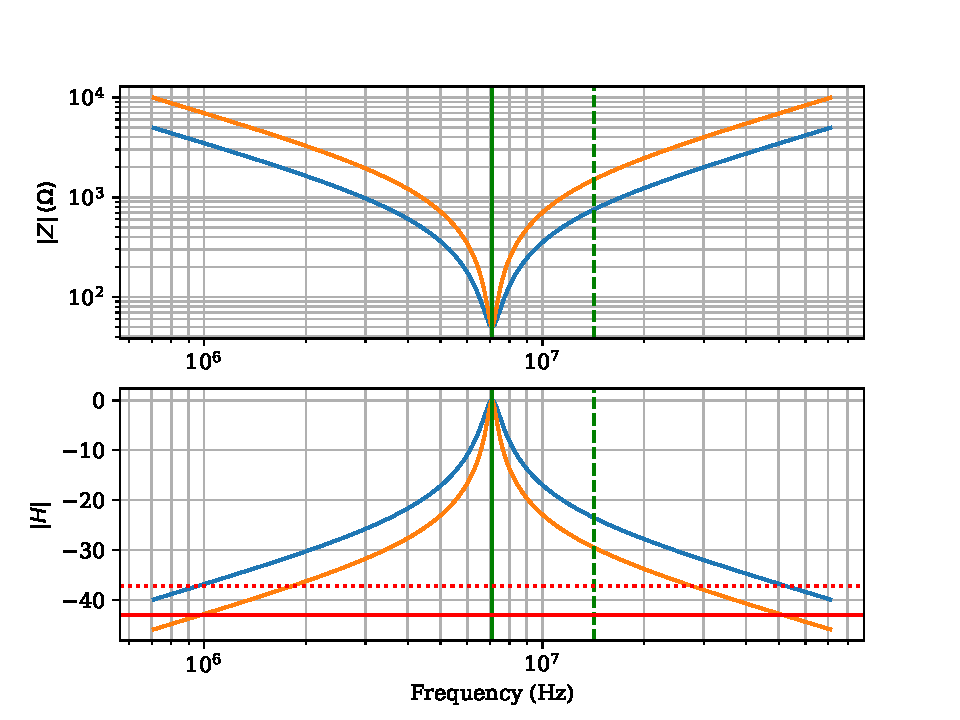
\includegraphics[width=.8\textwidth]{LCbp.pdf}
%\caption{Traditional LC bandpass filter for a Class E Amplifier for $Q=10$ (blue) and $Q=20$ (orange). Fundamental frequency is 7.1 MHz (green line), second harmonic at 14.2 MHz (dotted green line) are shown as vertical lines. FCC required attenuation of 43 dB (red line) and the target minimum harmonic suppression including Class E natural suppression of 5.7 dB (dotted red line). }
%\label{ClassEtradfiltmatchsimple}
%\end{figure}
%
%\subsubsection{``Power Boost" Class E}
%
%As seen in Table \ref{comparetable}, the standard design can output more power either by increasing $V_{CC}$ or decreasing the load resistance. We can use an LC circuit to decrease the load resistance, thereby boosting power (and doing some low-pass-filtering along the way).
%
%To increase output power and perform additional low-pass filtering, you can use an LC impedance transformer before the antenna. This lowers $R_L<R_{ant}$, and does not require an additional inductor since you can add the transformer inductor inductance to the existing inductor. The circuit is presented in Figure \ref{ClassEimptrans1}.
%
%\begin{figure}
%\centering
%\begin{circuitikz}
%  \draw (1,1) node[left]{$v_c$} to[C=$C_f$,o-]
%  (3,1) to[L=$L_{tot}$, name=Ltot]
%  (5,1) to[L=$L_{match}$, name=Lm]
%  (7,1) to[C=$C_2$]
%  (7,-1) node[tlground]{};
%  \draw  (7,1) -- (8.5,1)  to[R=$R_{ant}$]
%  (8.5,-1) node[tlground]{};
%  \node[rectangle, draw, dashed, fit=(Lm) (Ltot) (Lmlabel) (Ltotlabel)](box){};
%  \node[above] at (box.north){$L_2$};
%\end{circuitikz}
%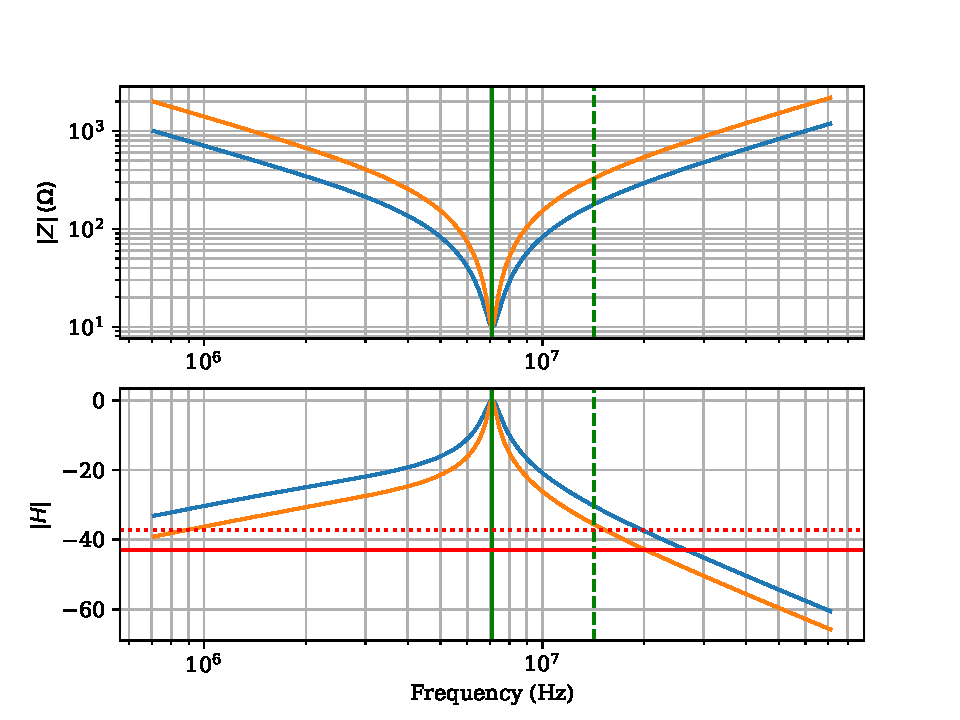
\includegraphics[width=.8\textwidth]{LCbpimp1.pdf}
%\caption{``Power Boosting" Impedance Transformer Class E with BPF. Both the transformer and BPF have the same $Q$: $Q=10$ (blue) and $Q=20$ (orange). $H$ is normalized to $1$ at $\omega$.}
%\label{ClassEimptrans1}
%\end{figure}
%
%First, determine how much power out ($P_{out}$) you'd like. From there you can find $C_2$ and $L_{match}$ usint a standard L-match circuit:
%
%\begin{align*}
%R_L&=\frac{0.58V_{CC}^2}{P_{out}}
%& Q &= \sqrt{\frac{R_{ant}}{R_L}-1}  \\
%%=\sqrt{\frac{R_{ant}{P_{out}}}{0.58V_{CC}^2}-1}\\
%L_{match}&=\frac{Q R_L}{\omega} & C_2&=\frac{Q}{R_{ant} \omega}
%\end{align*}
%
%Practically speaking, the load resistance should be at least $R_L>\SI{10}{\ohm}$ as to not draw too much current and avoid excessively large voltages on the filter components. Therefore, $1<Q<2$ and $P_{new}<5\times P_{orig}$. Figure \ref{ClassEimptrans1} shows that using a L-match $Q=2$, corresponding to $5\times$ higher output power with a BPF $Q=20$ gets really close to hitting the FCC requirements. However, that requires a $\SI{22}{\micro\henry}$ inductor, which is quite large. But it's possible!
%
%\subsubsection{Second Order ``Power Boosting" Impedance Transforming}
%
%If a simple L-network impedance transform doesn't get enough harmonic suppression, you can further boost the $Q$ of the low-pass filter by using a ``pi" or ``t" network. Circuit examples are given in Figure \ref{ClassEimptrans2}. 
%
%
%\begin{figure}
%\centering
%\begin{circuitikz}
%  \draw (3,1) node[left]{$v_c$} to[C=$C_f$,o-]
%  (4.5,1) to[L=$L_{tot}$, name=Lf]
%  (7,1) to[C=$C_2$,name=C2]
%  (7,-1) node[tlground](gnd1){};
%  \draw  (7,1) to[L=$L_2$, name=L2] (9,1) to[C=$C_3$,name=C3] (9,-1) node[tlground](gnd2){};
%  \draw (9,1)--(10.5,1)
%  to[R=$R_{ant}$] (10.5,-1) node[tlground]{};
%  \node[rectangle, draw, dashed, fit=(C2) (gnd1) (gnd2) (L2) (L2label) (C3label) (C3)](box){};
%  \node[above] at (box.north){Pi Network};
%\end{circuitikz}
%\begin{circuitikz}
%  \draw (3,1) node[left]{$v_c$} to[C=$C_f$,o-]
%  (4.5,1) to[L=$L_{tot}$, name=Lf]
%  (7,1) to[L=$L_2$, name=L2] (9,1) to[C=$C_2$,name=C3] (9,-1) node[tlground](gnd2){};
%  \draw (9,1) to[L=$L_3$, name=L3]
%  (11,1) to[R=$R_{ant}$] (11,-1) node[tlground]{};
%  \node[rectangle, draw, dashed, fit=(C2) (gnd1) (gnd2) (L2) (L2label) (L3label) (L3)](box){};
%  \node[above] at (box.north){Tee Network};
%  \node[rectangle, draw, dotted, fit =(Lf) (Lflabel) (L2) (L2label)](box2){};
%\end{circuitikz}
%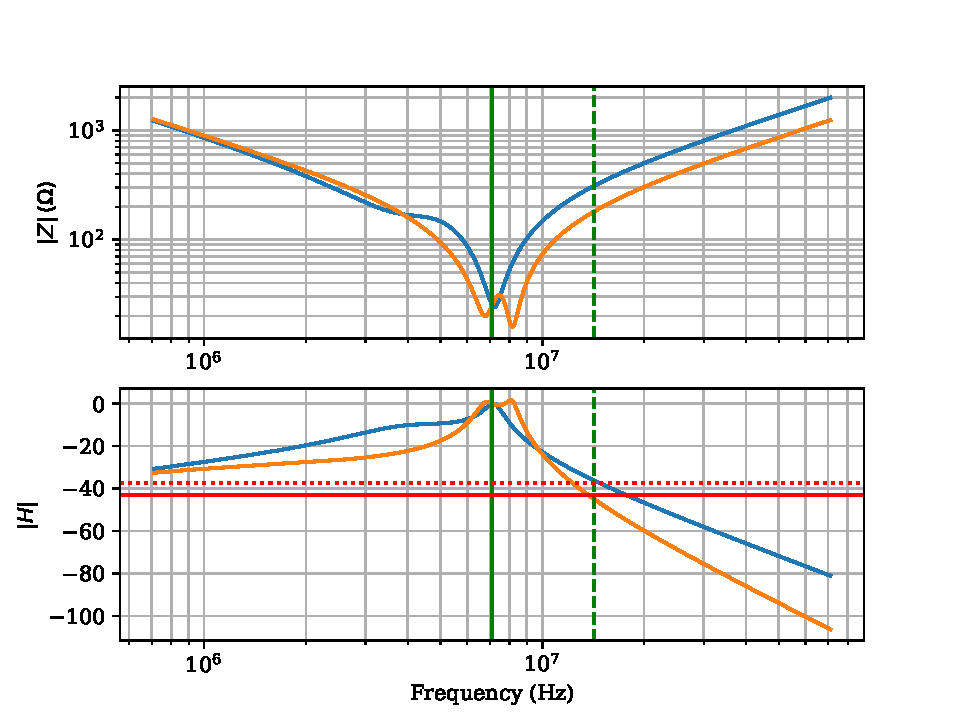
\includegraphics[width=0.8\textwidth]{LCbpimp2.pdf}
%\caption{Second Order ``Power Boosting" Impedance Transformer Class E, each with a $Q=5$ and $R_L=\SI{25}{\ohm}$. T-network in blue, pi-network in orange.}
%\label{ClassEimptrans2}
%\end{figure}
%
%Both configurations are low-pass filters that can ade that can be designed to make the load appear real and smaller than $R_{ant}$, thereby boosting power. So what choose one or the other? The answer is found by looking at the transfer curves and impedance plots for each circuit.
%
%Pi-networks present low impedances at high frequencies, t-networks present high impedances at high frequencies. We \textbf{\textit{need}} high impedances at high frequencies, so t-might bet a better typology! Pi-networks do have better harmonic suppression, however.
%
%The following sections shows how to calculate the values for the network.
%
%\subsubsection{Pi Matching}
%
%The pi network component values are calculated as follows:
%\begin{enumerate}
%\item Choose a $Q$ that meets your bandwidth need
%\item Find your desired apparent load resistance using $R_L=\frac{0.58 V_{CC}^2}{P_{out}}$
%\item Find the value of a virtual resistance $R_v$ that will each side of the pi-network will appear as:
%\begin{align*}
%Q&=\sqrt{\frac{R_L}{R_v}-1}+\sqrt{\frac{R_{ant}}{R_v}-1}\approx \sqrt{\frac{R_v}{R_L}-1}\\
%R_v&\approx R_L(Q^2+1)
%\end{align*}
%If you can use a computer to solve the un-approximated version, great - but the approximate one works OK too.
%\item Find the $Q$s corresponding to each side of the pi-network:
%\begin{align*}
%Q_1 & = \sqrt{\frac{R_L}{R_v}-1} &Q_2 &=\sqrt{\frac{R_{ant}}{R_v}-1}
%\end{align*}
%\item Find $C_2$, $C_3$, and $L_2$:
%\begin{align*}
%C_2 &= \frac{Q_1 R_L}{\omega } &C_3 &= \frac{Q_2 R_{ant}}{\omega } & L_2 = \frac{R_v}{\omega} (Q_1+Q_2)
%\end{align*}
%\end{enumerate}
%
%\subsubsection{T-Matching}: The tee network component values are calculated as follows:
%\begin{enumerate}
%\item Choose a $Q$ that meets your bandwidth need
%\item Find your desired apparent load resistance using $R_L=\frac{0.58 V_{CC}^2}{P_{out}}$
%\item Find the value of a virtual resistance $R_v$ that will each side of the t-network will appear as:
%\begin{align*}
%Q&=\sqrt{\frac{R_v}{R_L}-1}+\sqrt{\frac{R_v}{R_{ant}}-1}\approx \sqrt{\frac{R_v}{R_L}-1}\\
%R_v&\approx R_L(Q^2+1)
%\end{align*}
%Again, use a computer to solve this if you can, but the approximation is OK too.
%\item Find the $Q$s corresponding to each side of the t-network:
%\begin{align*}
%Q_1 & = \sqrt{\frac{R_v}{R_L}-1} &Q_2 &=\sqrt{\frac{R_v}{R_{ant}}-1}
%\end{align*}
%\item Find $L_2$,  $L_3$, and $C_2$
%\begin{align*}
%L_2 &= \frac{Q_1R_L}{\omega} &L_3 &= \frac{Q_2R_{ant}}{\omega} & C_2 = \frac{1}{R_v\omega}(Q_1+Q_2)
%\end{align*}
%\end{enumerate}
%
%
%
%\subsection{Pi- and T-Networks with Second Harmonic Notch Filters}
%
%To ensure that the second harmonic is properly suppressed (and impedance is zero), you can add capacitors in parallel to $L_2$ in a pi network or parallel to $L_3$ in a t network. This parallel LC branch can be tuned to $2\times \omega$ to eliminate the second harmonic. This is illustrated in Figure \ref{ClassEimpnotch}. Now both typologies reach the desired harmonic suppression levels and have higher impedances. \textbf{\textit{We've found designs suitable for easy QRP transmitters!}}
%
%
%\begin{figure}
%\centering
%\begin{circuitikz}
%  \draw (3,1) node[left]{$v_c$} to[C=$C_f$,o-]
%  (5,1) to[L=$L_{tot}$, name=Lf]
%  (7,1) to[C=$C_2$]
%  (7,-1) node[tlground]{};
%  \draw  (7,1) to[L, l_=$L_2$] (9,1) to[C=$C_3$] (9,-1) node[tlground]{};
%  \draw (9,1)--(10.5,1)
%  to[R=$R_{ant}$] (10.5,-1) node[tlground]{};
%  \draw (7,1) -- (7,2) to[C=$C_4$] (9,2) -- (9,1);
%\end{circuitikz}
%\begin{circuitikz}
%  \draw (3,1) node[left]{$v_c$} to[C=$C_f$,o-]
%  (4.5,1) to[L=$L_{tot}$, name=Lf]
%  (7,1) to[L=$L_2$, name=L2] (9,1) to[C=$C_2$,name=C3] (9,-1) node[tlground](gnd2){};
%  \draw (9,1) to[L, l_=$L_3$, name=L3]
%  (11,1) to[R=$R_{ant}$] (11,-1) node[tlground]{}
%  (9,1) -- (9,2) to[C=$C_3$] (11,2) -- (11,1);
%  \node[rectangle, draw, dotted, fit =(Lf) (Lflabel) (L2) (L2label)](box2){};
%  \node[above] at (box2.north) {$L_{tot'}$};
%\end{circuitikz}
%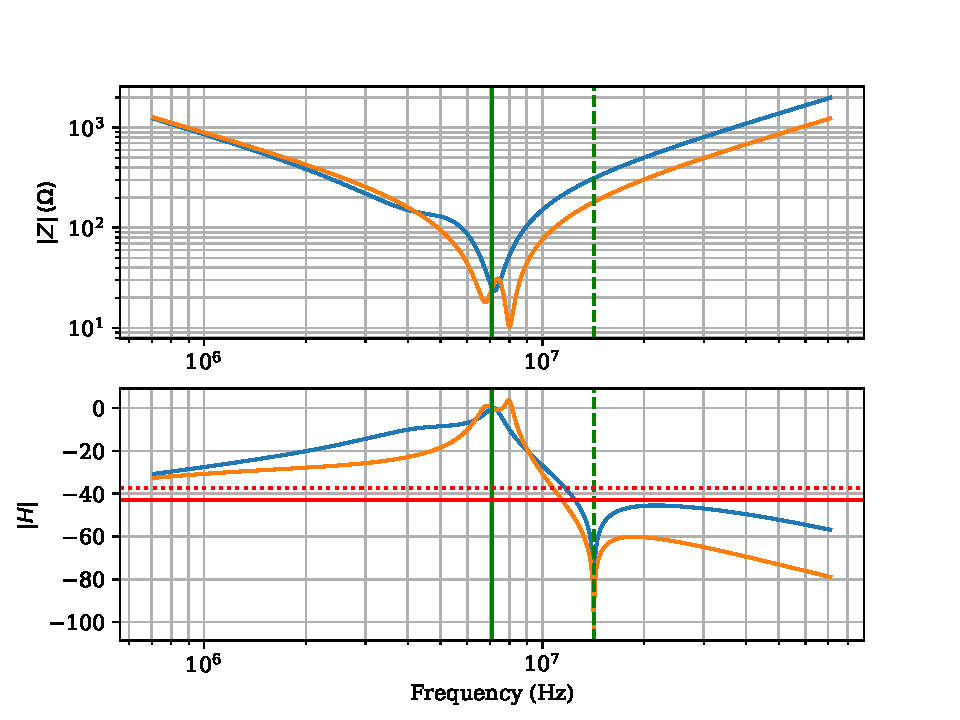
\includegraphics[width=.8\textwidth]{LCbpimp3.pdf}
%\caption{Notch Second Harmonic Pi- and T-Network Impedance Transformer Class E. T-network is blue, Pi-network is orange. Both with a $Q=5$ and $R_L=\SI{25}{\ohm}$.}
%\label{ClassEimpnotch}
%\end{figure}
%
%
%
%
%
%\subsection{QCX Class E}
%Finally we arrive at the QCX Class E. This actually is a completely different design and derivation (see section Section \ref{qcxdesign})! The standard equations don't hold because this entire design is based on not needing extra inductance to impedance match to $R_{ant}$, thereby simplifying the design since you can use off-the-shelf, well-known, broadband (low $Q$), completely real impedance matching filters. In fact, adding extra inductance (as required in ``normal" class E amplifiers) will \textbf{\textit{hurt}} QCX Class E performance. However, this approach does not have the theoretical 100\% efficiency found in the standard design (see derivations). The schematic is presented in Figure \ref{ClassEqcx}. While it is generally well performing, there are some drawbacks:
%
%\begin{enumerate}
%\item The filter is a bit overkill. Above showed that you can achieve needed performance with 1 fewer inductor and 2 fewer capacitors.
%\item The entire filter presents a short to ground at high frequencies. This hurts efficiency. However, QCX's Class E acutally reduces this downsides of this effect (see Section \ref{qcxdesign}). Nonetheless, it's not ideal.
%\end{enumerate}
%
%
%
%
%\section{Traditional Class E Amplifiers}\label{standarddesign}

%\begin{figure}
%\centering
%\begin{circuitikz}
%\draw
%(0,0) node[nigfetd](fet){}
%(fet.D) -- (0,1) to[short, i<=$i_t$] (1,1) to[short, i<=$i_s$] (3,1) to[L=$L_1$, i<=$i_l$] (3,3)
%  node[vcc](VCC){$V_{CC}$};
%  \draw (fet.S) -- (0,-1) node[ground]{};
%  \draw (fet.G) to[sqV] (fet.G -| -2,-2) -| (-2,-1)
%  node[ground]{};
%  \draw (1,1) to[C=$C_1$, i=$i_c$, v=$v_c$] (1,-1) node[ground]{};
%  \draw (3,1) to[short, i_=$i_{load}$] (4,1)
%  to[bandpass, l=Filter] (6,1) -- (7,1) to[R=$R_L$, v=$v_r$] (7,-1)
%  node[ground]{};
%\end{circuitikz}
%\caption{Generic Class E Amplifier}
%\label{ClassE}
%\end{figure}
%
%All Class E amplifiers generally have the same structure (with a few exceptions), shown in \ref{ClassE}. The basic structure consists of:
%\begin{itemize}
%\item A MOSFET is switched on and off by a pulsed voltage source applied to its gate. The fluctuating switch causes the voltage $v_c$ to fluctuate, and current to flow through $i_l$, $i_c$, and $i_{load}$.
%\begin{itemize}
%\item When the switch is closed: current flows through $i_t$ and and voltage at the node connected the filter, $L_1$, $C_1$, and transistor drain is grounded (i.e., $v_c=0$).
%\item When the switch is open: no current flows through the transistor should be close to zero ($i_t=0$)
%\end{itemize}
%\item A filter is placed such that $V_r$ is purely a single harmonic. The FCC requires 43 dB suppression of higher harmonics.
%\end{itemize}
%
%That's it! Everything then becomes a trade off between choosing values for the different components and designing a filter so the whole system can work together. Ideally, Class E amplifiers are 100\% efficient since the only places where current flows across a power dissipating element is the load resistor (antenna). While parasitic capacitances, inductances, and real resistances in all components make ideal efficiency impossible, achieving $>90\%$ efficiency is common.
%
%To demonstrate how the QCX Class E works, we first can quickly review a traditional Class E amplifier. Here's the traditional steps to analyze the circuit to derive component values:
%
%\begin{enumerate}
%\item Start by saying we'll make $L_1$ really large (much larger than the inductance of the load), thus making it an RF choke that lets DC pass through but blocks all AC signals. Therefore $i_l=I_{DC}$
%\item Next, we say that the filter only allows frequency $\omega = 2\pi f$ to pass through it, it's a perfect band pass filter that essentially has zero impedance at $\omega$ and infinite impedance at all harmonics and DC. Therefore we can write $i_{load}=a\sin(\omega t)+ b\cos(\omega t)$.
%\item Now that we know $i_{load}$ and $i_l$, we can find the current in the switching capacitor branch which is simply $i_s=I_{DC}-a\sin(\omega t)- b\cos(\omega t)$.
%\item Using $i_s$, we can find the voltage across the capacitor. We'll say the switch is closed from time $t=0$ to $\pi \omega$, and the switch is opened from $t=\pi/ \omega$ to $2 \pi / \omega$. Therefore:
%\begin{align*}
%t=0\rightarrow \pi/\omega: && v_c &=0\\
%t=\pi/\omega \rightarrow 2\pi/\omega: &&v_c &=\frac{1}{C_1}\int_{\pi/\omega}^{t} i_c\,dt'=\frac{1}{C_1}\int_{\pi/\omega}^{t} i_s\,dt'\\
%&& &= \frac{1}{C_1}\int_{\pi/\omega}^{t} I_{DC}-a\sin(\omega t')- b\cos(\omega t')\,dt'\\
%&& &= \frac{1}{\omega C_1}\left[ I_{DC}\left(\omega t- \pi \right)+a \cos(\omega t)+ a - b \sin(\omega t) \right] \\
%\end{align*}
%We know the switch is closed at $\omega t=2\pi$, so the voltage should be zero then. Therefore:
%\begin{align*}
%0 &= \frac{1}{\omega C_1}\left[ \pi I_{DC}+2a \right]\\
%a &= -\frac{\pi}{2} I_{DC}
%\end{align*}
%We also can say we want the first derivative of the voltage to be zero when the switch is first closed for maximum efficiency.
%\begin{align*}
%\frac{dv_c}{dt}\Bigr|_{t=2\pi/\omega}=0 &=  \frac{1}{C_1}\left[ I_{DC}+\frac{\pi}{2} I_{DC}\sin(\omega t)- b\cos(\omega t) \right]\Bigr|_{t=2\pi/\omega}\\
%b&=I_{DC}
%\end{align*}
%Therefore:
%\begin{align*}
%t=0\rightarrow \pi/\omega: \quad && v_c &=0\\
%t=\pi/\omega \rightarrow 2\pi/\omega: \quad &&v_c &=\frac{I_{DC}}{\omega C_1}\left[ \left(\omega t-\frac{3\pi}{2}\right)-\frac{\pi}{2} \cos(\omega t)-\sin(\omega t) \right] \\
%\end{align*}
%and
%\begin{align*}
%i_{load}&=I_{DC}\left( -\frac{\pi}{2}\sin(\omega t)+ \cos(\omega t)\right)\\
%&\approx I_{DC} \left( 
%\frac{\sqrt{\pi^2+4}}{2}\cos
% \left( \omega t-57.5^\circ
% \right)
%\right)
%\end{align*}
%
%
%We can plot $v_c$ and see that the voltage is zero when the switch is closed (first half of the period the capacitor in grounded), then it increases and returns to zero right before the switch closes again in Figure \ref{vcplot}. We can now also plot what current $i_s$ is doing through the cycle in Figure \ref{isplot}.
%
%
%
%\begin{figure}
%\centering
%\begin{tikzpicture}
%\begin{axis}[
%%    axis lines = left,
%    xlabel = {Time ($2\pi/\omega)$},
%    ylabel = {$v_c/V_{CC}$},
%    grid=both
%]
%\addplot [
%    domain=0:.5, 
%    samples=100, 
%    ]
%    {0*x};
%\addplot [
%    domain=.5:1, 
%    samples=100, 
%]
%{pi*( x*2*pi-3*pi/2-pi/2*cos(deg(x*2*pi))-sin(deg(x*2*pi)))};
%
%\end{axis}
%\end{tikzpicture}
%\caption{Capacitor voltage versus time for one switch period.}
%\label{vcplot}
%\end{figure}
%
%
%\begin{figure}
%\centering
%\begin{tikzpicture}
%\begin{axis}[
%%    axis lines = left,
%    xlabel = {Time ($2\pi/\omega)$},
%    ylabel = {$i_t / I_{DC}$},
%    grid=both
%]
%\addplot [
%    domain=0:.5, 
%    samples=100, 
%    color=red
%    ]
%    {1+pi/2*sin(deg(x*2*pi))-cos(deg(x*2*pi))};
%\addplot [
%    domain=.5:1, 
%    samples=100, 
%    color=red,
%    ] coordinates{(.5,2) (.5,0) (1,0)};
%
%\end{axis}
%\end{tikzpicture}
%
%\begin{tikzpicture}
%\begin{axis}[
%%    axis lines = left,
%    xlabel = {Time ($2\pi/\omega)$},
%    ylabel = {$i_c/I_{DC}$},
%    grid=both
%]
%\addplot [
%    domain=0:5, 
%    samples=100, 
%    color=blue,
%    ] coordinates{(0,0) (.5,0) (.5,2)};
%\addplot [
%    domain=.5:1, 
%    samples=100, 
%    color=blue
%]
%{1+pi/2*sin(deg(x*2*pi))-cos(deg(x*2*pi))};
%
%\end{axis}
%\end{tikzpicture}
%\caption{Transistor source current (top) and capacitor current (bottom) over one switch period.}
%\label{isplot}
%\end{figure}
%
%\item We've had $I_{DC}$ hanging around for a while, but we don't really know what it is. To find it, we can realize that the power in to the circuit only comes fro $V_{CC}$, and the power is only dissipated in $R_L$, therefore those two powers must be equal.
%
%\begin{align*}
%P = V_{CC}I_{DC}&=\frac{1}{2}|i_{load}|^2 R_L=\frac{4+\pi^2}{8}I_{DC}^2 R_L\\
%I_{DC}&=\frac{8}{4+\pi^2}\frac{V_{CC}}{R_L}\\
%P&=\frac{8}{4+\pi^2}\frac{V_{CC}^2}{R_L}
%\end{align*}
%
%The conclusion here is the \textbf{you can increase output power} by either increasing supply voltage, or by using an impedance transforming network to reduce an antenna's load from 50~$\Omega$ to something less (usually around 10~$\Omega$)
%
%\item Now we know all the currents in the circuits at all time and the voltage across the capacitor, inductor, transistor drain to source, and presented to the filter. The last step is to figure out what filter we need to both remove unwanted frequency components and impedance matching to our load.
%
%We know the voltage $v_c$ and the current $i_{load}$, so our filter just is something with the impedance $Z_{filt}=\frac{v_c}{i_{load}}$. We know $i_{load}=0$ for all frequencies except the harmonic, therefore $Z_{filt}(\omega)=\infty$ for all frequencies except the one we want. This is a crucial part of Class E design. Sometimes people think the filter is just there to filter out frequencies from reaching the antenna when in fact it is there \textbf{to stop those currents from even flowing out of the input node in the first place!}
%
%Now that we know what we want in the frequency domain, we can look at what $v_c$ looks like in the frequency domain by representing $v_c$ as the sum of sine and cosine functions (write it as a ``Fourier Series").
%
%\begin{multline*}
%v_c = \frac{8}{4+\pi^2}\frac{V_{CC}}{\omega C_1 R_L} \Big( \frac{1}{\pi}-\frac{1}{2}\sin(\omega t)-\frac{\pi^2-8}{4\pi}\cos(\omega t)\\
%+\frac{1}{6}\sin(2\omega t)-\frac{2}{3\pi}\cos(2\omega t)+\frac{2}{9\pi}\cos(3\omega t)+\cdots \Big)
%\end{multline*}
%and as a reminder
%\begin{align*}
%i_{load}&=\frac{8}{4+\pi^2}\frac{V_{CC}}{R_L}\left( -\frac{\pi}{2}\sin(\omega t)+ \cos(\omega t)\right)
%\end{align*}
%
%So the filter design begins to pop up out:
%\begin{itemize}
%\item We need a DC blocking capacitor since there is a DC component in $v_c$ and none in $i_{load}$.
%\item We'd want an infinite impedance at $2\omega t$. That's possible with a notch filter. But even if we don't use a notch filter, if we can get it 30 dB less than the fundamental, we're doing pretty good (at least from the FCC's point of view). The voltage is already smaller than the fundamental by a factor of:
%\begin{align*}
%\frac{\left| v_c(2\omega)\right|}{|v_c(\omega)|}=\frac{\sqrt{  \left(\frac{1}{6}\right)^2+\left(\frac{2}{3\pi}\right)^2}}{\sqrt{\left( \frac{1}{2} \right)^2+\left(\frac{\pi^2-8}{4\pi} \right)^2}}
%\approx 0.52
%\approx -5.7 \text{ dB}
%\end{align*}
%
%\textbf{So the filter, practically, really only needs to do 25 dB of filtering to be sufficient}, which is exactly what NM0S saw when he experimentally measured and designed his Class E.
%
%Now that we know what we want for the higher harmonics, we can turn our attention to the fundamental frequency $\omega$
%
%
%\end{itemize}
%\begin{align*}
%v_c &= \frac{8}{4+\pi^2}\frac{V_{CC}}{\omega C_1 R_L} \left( -\frac{1}{2}\sin(\omega t)-\frac{\pi^2-8}{4\pi}\cos(\omega t)\right)\\
%i_{load}&=\frac{8}{4+\pi^2}\frac{V_{CC}}{R_L}\left( -\frac{\pi}{2}\sin(\omega t)+ \cos(\omega t)\right)
%\end{align*}
%
%It turns out that if our filter acts like an inductor in series with our load resistor $R_L$ (representing our antenna), we can get $v_c$ and $i_r$ to ``line up" with each other so that we can get ideal, perfect matching and theoretically achieve 100\% efficiency! This is seen in Figure \ref{ClassEtradmatch}.
%
%\begin{figure}
%\centering
%\begin{circuitikz}
%  \draw (3,1) node[left]{$v_c$} to[short, i_=$i_{load}$,o-] (4,1)
%  to[bandpass, l=Perfect BPF] (6,1) to[L=$\Delta L$] (8,1) to[R=$R_L$, v=$v_r$] (8,-1)
%  node[ground]{};
%\end{circuitikz}
%\caption{Traditional impedance matching for a Class E Amplifier}
%\label{ClassEtradmatch}
%\end{figure}
%
%We can then find what $\Delta L$ needs to be.
%
%\begin{align*}
%v_c &=\omega \Delta L \frac{di_{load}}{dt}+i_{load}R_L\\
%% &=\frac{8}{4+\pi^2}\frac{V_{CC}}{R_L}\left( \omega \Delta L \left( -\frac{\pi}{2}\cos(\omega t)- \sin(\omega t)\right) +R_L\left( -\frac{\pi}{2}\sin(\omega t)+ \cos(\omega t)\right)\right)\\
%&=\frac{8}{4+\pi^2}\frac{V_{CC}}{R_L}
%\left[ \left(-\omega \Delta L-\frac{R_L\pi}{2}\right)\sin(\omega t)+\left(- \frac{\omega \Delta L\pi}{2}+R_L\right)\cos(\omega t)\right]\\
%v_c &= \frac{8}{4+\pi^2}\frac{V_{CC}}{\omega C_1 R_L} \left( -\frac{1}{2}\sin(\omega t)-\frac{\pi^2-8}{4\pi}\cos(\omega t)\right)\\
%\end{align*}
%
%Set those bottom two lines equal to each other and you'll find expressions for $\Delta L$ and $C_1$.
%
%\begin{align*}
%\Delta L &=\frac{\pi(\pi^2-4)R_L}{16\omega}\approx  \frac{1.1525 R_L}{\omega}\\
%C_1 & = \frac{1}{\omega R_L}\frac{8}{\pi(4+\pi^2)}\approx \frac{1}{5.4466 \omega R_L}
%\end{align*}
%
%Which also gives us an even simpler expression for $v_c$.
%
%\begin{align*}
%v_c &=0 &t&=0\rightarrow \pi/\omega\\
%v_c &= \pi V_{CC} \left[ \left(\omega t-\frac{3\pi}{2}\right)-\frac{\pi}{2} \cos(\omega t)-\sin(\omega t) \right] &t&=\pi/\omega \rightarrow 2\pi/\omega\\ \\
%v_c &= V_{CC}\Big( 1-\frac{\pi}{2}\sin(\omega t)-\frac{\pi^2-8}{4}\cos(\omega t) &&\text{Fourier Series}\\
%&\qquad +\frac{\pi}{6}\sin(2\omega t)-\frac{2}{3}\cos(2\omega t)+\frac{2}{9}\cos(3\omega t)+\cdots \Big)
%\end{align*}
%
%\item Next we can revist ``how big does $L_1$ need to be?" We just said it has to be big - how big? Basically we want the current through $L_1\approx I_{DC}$, which means we want all the other frequency components to be much less than $I_{DC}$. So what is the current through $L_1$?
%
%Basically, we know that the current through $L_1$ is going to have a DC component and some AC. We just want the DC component to be much larger than the AC. So let's calculate the current through $L_1$!
%\begin{align*}
%i_l &= \frac{1}{L_1}\int V_{CC}-v_c\,dt\\
%&= \frac{1}{L_1}\int V_{CC}- V_{CC}\Big( 1-\frac{\pi}{2}\sin(\omega t)-\frac{\pi^2-8}{4}\cos(\omega t)\\
%&\qquad +\frac{\pi}{6}\sin(2\omega t)-\frac{2}{3}\cos(2\omega t)+\frac{2}{9}\cos(3\omega t)+\cdots \Big)\,dt\\
%&= I_{DC}+\frac{V_{CC}}{\omega L_1}\Big(-\frac{\pi}{2}\cos(\omega t)+\frac{\pi^2-8}{4}\sin(\omega t)\\
%&\qquad+\frac{\pi}{12}\cos(2\omega t)+\frac{1}{3}\sin(2\omega t)+\frac{2}{27}\sin(3\omega t)-\cdots \Big)
%\end{align*}
%
%So we want $L_1$ to be large enough such that the magnitude of the largest AC components of $i_L$ is much less than $I_{DC}$. By inspection, the $\omega$ component (fundamental frequency) is the largest, therefore
%
%\begin{align*}
%I_{DC} &\gg \frac{V_{CC}}{\omega L_1} \sqrt{\left(\frac{\pi}{2}\right)^2+\left(\frac{\pi^2-8}{4}\right)^2}\\
%\frac{8}{4+\pi^2}\frac{V_{CC}}{R_L} &\gg \frac{V_{CC}}{\omega L_1} \frac{\sqrt{\pi^4-12\pi^2+64}}{4}\\
%\frac{V_{CC}}{1.73 R_L} &\gg 1.64 \frac{V_{CC}}{\omega L_1}\\
%L_1 &\gg 2.84 \frac{R_L}{\omega}
%\end{align*}
%
%\item Finally, we can choose the filter. We want a filter with infinite impedance at all frequencies except at our chosen frequency. An inductor and capacitor in series does that, like in Figure \ref{ClassEtradfiltmatch}.
%
%\begin{figure}
%\centering
%\begin{circuitikz}
%  \draw (3,1) node[left]{$v_c$} to[C=$C_f$, i>_=$i_{load}$,o-] (5,1)
%  to[L=$L_f$, name=Lf] (7,1) to[L=$\Delta L$, name=DL] (9.5,1) to[R=$R_L$, v=$v_r$] (9.5,-1)
%  node[ground]{};
%    \node[rectangle, draw, dashed, fit=(DL) (Lf) (DLlabel) (Lflabel)](box){};
%    \node [above, align=center] at (box.north) {$L_{tot}$};
%\end{circuitikz}
%\caption{Traditional filter with impedance matching for a Class E Amplifier}
%\label{ClassEtradfiltmatch}
%\end{figure}
%
%Theoretically, you want a perfect filter with infinitesimal bandwidth ($\Delta \omega$. The ratio of a filter's frequency to its bandwidth is a filter's $Q=\frac{\omega}{\Delta \omega}$, so you'd like an infinite $Q$. For a given $Q$, you can therefore find $C_f$ and $L_f$ in Figure \ref{ClassEtradfiltmatch}:
%
%\begin{align*}
%Q_f &=\frac{\omega L_f}{R_L}\\
%L_f &=\frac{Q_f R_L}{\omega} \\
%C_f &= \frac{1}{\omega^2 L_f}=\frac{1}{Q_f R_L \omega}\\
%L_{tot} & = L_f+\Delta L=\frac{R_L}{\omega}\left(Q_f+1.1525\right)
%\end{align*}
%
%Although we want $Q_f=\infty$, this whole approach works well for $Q_f>10$ or so. In fact, if you use a $Q\approx 20$, you can achieve 30 dB suppression with just that single inductor! However, tuning that LC circuit will be tricky, experimentally.  For lower $Q_f$, check out [REFERENCE] for equations to ``correct" for imperfect $Q_f$.\footnote{As a note, that paper decreases capacitance rather than increases inductance which has the same effect. Also, they use $Q_L$ instead of $Q_f$, which includes the extra impedance matching.}
%
%\end{enumerate}
%


\section{QCX Design}\label{qcxdesign}
There are a lot of Class E explanation documents on the internet, but I haven't found a caparison document intended for people just wanting to figure out what's the deal with different Class E amplifiers they are seeing.

This was motivated by discussions at the $\mu$SDX project where different builds were using different Class E designs that were incompatible with each other (one required inductive loads, one required only real loads). Having a base transceiver design with completely different PA filter requirements could cause problems if people tried to ``mix-and-match" filters between the two.

When considering this, I saw that there was no theoretical description of the qrp-labs QCX Class E amplifier that was used by several people. The qrp-labs.com's ``QCX" transceiver\footnote{\url{https://qrp-labs.com/qcxp}} has an unconventional Class E amplifier design. The designer, Hans Summers (G0UPL) described the design as sort of a trial and error process guided by some ideas. It turned out that it worked pretty well, but it sort of violated some ``traditional" class E amplifier design rules. I decided to model it in ngspice to figure out what's going on, and found that it is actually a beautiful and elegant design that is fundamentally different than the strategies of other class E amplifiers. Some may call it "ghetto," but there's an elegance to it how it performs.

\subsection{QRP-Labs Design}
The QCX manual says to use the following approach to choose components in Figure \ref{ClassE}. Although not grounded in theory, but in experimental trial and error - and produces excellent results!
\begin{enumerate}
\item Choose $L_1=R_{ant}/\omega$
\item Choose $C_1=1/(\omega R_{ant} )$
\item For the filter, use Figure \ref{ClassEqcx} and values from G-QRP club's technical pages, originally designed by Ed Whetherhold (W3NQN).
\item Tweak the value of $C_1$ to get the highest efficiency. This is the key point - and why it works so well. Experimental tinkering is often is superior to theory!
\end{enumerate}


\begin{figure}
\centering
\begin{circuitikz}
\draw
(0,0) node[nigfetd](fet){}
(fet.D) -- (0,1) to[short, i<=$i_t$] (1,1) to[short, i<=$i_s$] (3,1) to[L=$L_1$, i<=$i_l$] (3,3)
  node[vcc](VCC){$V_{CC}$};
  \draw (fet.S) -- (0,-1) node[ground]{};
  \draw (fet.G) to[sqV] (fet.G -| -2,-2) -| (-2,-1)
  node[ground]{};
  \draw (1,1) to[C=$C_1$, i=$i_c$, v=$v_c$] (1,-1) node[ground]{};
  \draw (3,1) to[short, i_=$i_{load}$] (4,1)
  to[bandpass, l=Filter] (6,1) -- (7,1) to[R=$R_L$, v=$v_r$] (7,-1)
  node[ground]{};
\end{circuitikz}
\caption{Generic Class E Amplifier}
\label{ClassE}
\end{figure}

\subsection{Analytical Approach to QCX Class E Design}
Modelling the QCX Class E with the values qrp-labs uses allows you to analyze the voltages at the different nodes in order to come up with a theoretical approach to help design and optimize this style of Class E amplifier. Below is the outcome of that approach:

\begin{enumerate}
\item The starting point is the expression for $v_c$. The qrp-labs $v_c$ is symmetric, which is needed because there is no LC bandpass filter. The voltage at $v_c$ actually closely follows:
\begin{align*}
t&=0\rightarrow \pi/\omega: &v_c &= 0\\
t&=\pi/\omega\rightarrow2\pi/\omega: &v_c &= A\sin^2(\omega t)\\
& & &=A\left(\frac{1}{2}-\frac{1}{2}\cos(2\omega t)\right)
\end{align*}
Acknowledging that the average voltage at $\left\langle v_c \right\rangle = V_{CC}$, you can find $A$:
\begin{align*}
V_{CC}&=\frac{1}{2\pi/\omega}\int_0^{2\pi/\omega}v_c\,dt'\\
V_{CC}&=\frac{1}{2\pi/\omega}\int_{\pi/\omega}^{2\pi/\omega}A\left(\frac{1}{2}-\frac{1}{2}\cos(2\omega t)\right)\,dt\\
4V_{CC}&=A\\
\end{align*}
Allowing us to write $v_c$ as a simple expression seen in Figure \ref{QCXvcplot} and equations below. It's evident that $v_c$ is zero at switch turn on and off, with zero derivative at turn on and off as well.
\begin{align*}
t&=0\rightarrow \pi/\omega: &v_c &= 0\\
t&=\pi/\omega\rightarrow2\pi/\omega: &v_c &= 2V_{CC}-2V_{CC}\cos(2\omega t)
\end{align*}
\begin{figure}
\centering
\begin{tikzpicture}
\begin{axis}[
%    axis lines = left,
    xlabel = {Time ($2\pi/\omega)$},
    ylabel = {$v_c/V_{CC}$},
    grid=both
]
\addplot [
    domain=0:.5, 
    samples=100, 
    ]
    {0*x};
\addplot [
    domain=.5:1, 
    samples=100, 
]
{2-2*cos(deg(x*4*pi))};

\end{axis}
\end{tikzpicture}
\caption{QCX capacitor voltage versus time for one switch period.}
\label{QCXvcplot}
\end{figure}


\item Now we can find the current through the capacitor for the time period $t=\pi/\omega\rightarrow2\pi/\omega$ as seen in Figure \ref{QCXicplot} and below:
\begin{align*}
i_c &= C_1 \frac{d v_c}{dt}=4 \omega C_1 V_{CC}  \sin(2\omega t)\\
\end{align*}

\begin{figure}
\centering
\begin{tikzpicture}
\begin{axis}[
%    axis lines = left,
    xlabel = {Time ($2\pi/\omega)$},
    ylabel = {$i_c/(\omega C_1 V_{CC})$},
    grid=both
]
\addplot [
    domain=0:.5, 
    samples=100, 
    ]
    {0*x};
\addplot [
    domain=.5:1, 
    samples=100, 
]
{4*sin(deg(x*4*pi))};

\end{axis}
\end{tikzpicture}
\caption{QCX capacitor current versus time for one switch period.}
\label{QCXicplot}
\end{figure}

\item Next we'll find the current through the load (antenna). QCX Class E amplifiers use a filter that presents an entirely real load to the amplifier, and the blocking capacitor $C_f$ in Figure \ref{ClassEqcx} is chosen such that $C_f < \frac{1}{R_{ant}\omega}$. To find the current through the load we represent $v_C$ as a Fourier series:
\begin{align*}
v_c &= V_{CC}-\frac{ 16}{3\pi}V_{CC}\sin(\omega t)-V_{CC}\cos(2\omega t) + \frac{ 16}{15\pi}V_{CC}\sin(3\omega t)+\cdots\\
\end{align*}
We also can present $R_L$ as a complex impedance as a function of frequency ($Z(\omega')$) since it is the combined impedance of the filter with the antenna. The filter presents a real load at the fundamental frequency ($\omega$), so $Z(\omega)=R_{ant}$. The DC blocking capacitor makes $Z(0)=\infty$, but $Z$ can by anything at other frequencies. Typically, Class E amplifiers want filters that have $Z(n\omega)=\infty$ for all $n\neq 1$, however, QCX Class E is "special" as we will see.
\begin{align*}
i_{load}&=\frac{v_c}{Z(\omega')}\\
&= -\frac{ 16}{3\pi}\frac{ V_{CC}}{R_{ant}} \sin(\omega t)-\frac{V_{CC}}{Z(2\omega)}\cos(2\omega t) + \frac{ 16}{15\pi}\frac{V_{CC}}{Z(3\omega)}\sin(3\omega t)+\cdots
\end{align*}
From which you can find the average RF power emitted:
\begin{align*}
\left\langle P_{out} \right\rangle = \frac{ 128}{9\pi^2} \frac{ V_{CC}^2}{R_{ant}}\approx 1.44\frac{ V_{CC}^2}{R_{ant}}
\end{align*}

\item Next we find the current through the inductor, which has the form as seen in Figure \ref{QCXilplot} and derived below:
\begin{align*}
& &i_l&=\frac{1}{L_1}\int_{-\infty}^t V_{CC}-v_c\, dt'\\
t&=0\rightarrow \pi/\omega: &i_l&=i_{l0} +\frac{1}{L_1}\int_{0}^t V_{CC}\, dt' \\
& &&=i_{l0}+\frac{V_{CC}}{\omega L_1}\omega t\\
t&=\pi/\omega\rightarrow 2\pi/\omega: &i_l&=i_{l0} +\frac{1}{L_1}\int_{0}^{\pi/\omega} V_{CC}\, dt' +\frac{1}{L_1}\int_{\pi/\omega}^t V_{CC}-v_c\, dt'\\
& &&=i_{l0}+\frac{V_{CC}}{\omega L_1}\left(2\pi-\omega t+\sin(2\omega t)\right)\\
\end{align*}
Which has the form as seen in Figure \ref{QCXilplot}.
\begin{figure}
\centering
\begin{tikzpicture}
\begin{axis}[
%    axis lines = left,
    xlabel = {Time ($2\pi/\omega)$},
    ylabel = {($i_l-i_{l0})/(V_{CC}/\omega L)$},
    grid=both
]
\addplot [
    domain=0:.5, 
    samples=100, 
    ]
    {x*2*pi};
\addplot [
    domain=.5:1, 
    samples=100, 
]
{2*pi-(x*2*pi)+sin(deg((x*2*pi)*2))};

\end{axis}
\end{tikzpicture}
\caption{QCX inductor current versus time for one switch period.}
\label{QCXilplot}
\end{figure}

The $i_{l0}$ term can be found be equating in the input and output average powers. The input voltage is $V_{CC}$, and the input current is $I_{DC}=\frac{1}{2\pi/\omega}\int_0^{2\pi/omega}i_l\, dt'$
\begin{align*}
\left\langle P_{in} \right\rangle &= \left\langle P_{out} \right\rangle\\
\frac{V_{CC}}{2\pi/\omega}\int_0^{2\pi/\omega} i_l \, dt'&=\frac{128}{9\pi^2}\frac{V_{CC}^2}{R_{ant}}\\
i_{l0}&=\frac{V_{CC}}{R_{ant}}\left(\frac{128}{9\pi^2}-\frac{\pi R}{2 L\omega}\right)
\end{align*}


\item To bring it all together, we have to make sure the currents all equal to each other. We'll have to find the values of $L_1$, $C_1$ that make it happen. When the switch is closed:
\begin{align*}
t&=0\rightarrow \pi/\omega: &i_l&=i_{load}+i_t
\end{align*}
And since $i_t$ can take any current (it's a short to ground!) we don't have to worry about that. The interesting thing is when the switch is closed:
\begin{align*}
t&=\pi/\omega\rightarrow 2\pi/\omega: &i_l=i_{load}+i_c
\end{align*}
To match these currents, we'll make the fundamental component of the Fourier series of each current equal to each other when the switch is open. When the switch is closed, $i_l-i_c-i_{load}-i_t=0$ is guaranteed since  $i_t$ can provide enough current to balance the other three. However, when the switch is closed, $i_t=0$ and the three other currents must be equal. Therefore, we'll make sure the fundamental component of the Fourier series of $i_l-i_c-i_{load}-i_t=0$ at all time.

\begin{align*}
t&=0\rightarrow\pi/\omega: &0&=i_{l1}-i_{c1}-i_{load1}-i_{t1}\\
t&=\pi/\omega\rightarrow 2\pi/\omega: &0&=i_{t2}-i_{c2}-i_{load2}
\end{align*}
Where 1 and 2 denote real values for the first or second half of the cycle, respectively, and zeros for the other half. For the second half of the cycle, we must find $L_1$, $C_1$ that makes the following true.
\begin{align*}
I(t)=0=i_{l0}&+\frac{V_{CC}}{\omega L_1}\left(2\pi-\omega t+\sin(2\omega t)\right)\\
&-4\omega C_1 V_{CC}\sin(2 \omega t)\\
&+\Big( \frac{16V_{CC}}{3\pi R_{ant}}\sin(\omega t)+\frac{V_{CC}\Re\left\{Z(2\omega)\right\}}{|Z(2\omega)|^2}\cos(2\omega t)\\
&\quad +\frac{V_{CC}\Im\left\{Z(2\omega)\right\}}{|Z(2\omega)|^2}\sin(2\omega t)+\cdots \Big)\\
\end{align*}



If $Z(2\omega)$ is large $Z(2\omega)\gg\frac{R_{ant}}{4}$:
\begin{align*}
\frac{1}{L_1C_1}=(2\omega)^2\\
L_1=\frac{3 \pi R_{ant} }{8\omega}
\end{align*}

If Z2w is real (like in QCX!):
\begin{align*}
\frac{1}{L_1C_1}=(2\omega)^2\\
L_1=\frac{3 \pi R_{ant} Z(2\omega) }{[2R_{ant}+8Z(2\omega)]\omega}
\end{align*}

Generally:
\begin{align*}
C_1 = \frac{\Im\{Z(2\omega)\}L_1\omega+|Z(2\omega)|}{4L_1 |Z(2\omega)|w^2}\\
L_1=\frac{3 \pi R_{ant} \Re\{Z(2\omega)\} |Z(2\omega)| }{[2R_{ant}|Z(2\omega)|+8\Re\{Z(2\omega)\}]\omega}
\end{align*}

\textbf{impedance of filter matters}. if second harmonic is completely real, above works. If capacitive at 2w (as in pi networks, negative 90 degrees), cos(2w) turns into -sin(2w), and it modifies your capacitance. (not derived here)

Finally, there is a DC component to $I(t)$ when the switch is closed that needs to be accounted for. How this is handled is by making sure $C_f \gg C_1$ and $C_f \gg C_2$. This means that the current will charge up the capacitor $C_f$ while not affecting $v_c$ that much. When the switch is closed, the current will discharge out of $C_f$ to ground. A $C_f\approx \SI{100}{\nano\farad}$ seems to work well.



\end{enumerate}

\end{document}